\documentclass[../main.tex]{subfiles}
% !TeX root = ../main.tex
\begin{document}
	\section{Financial Statement Analysis}
	
	Financial statement analysis applies analytical tools to general-purpose 
	financial statements and related data for making business decisions.  It 
	provides us an effective and systematic basis for making business 
	decisions. These techniques help us to better understand the company and 
	reduce uncertainty associated with financial information.
	
	
	Financial statement analysis is used by many people within the 
	organization. Managers find financial analysis helpful in planning and 
	controlling operations. External users of financial statements are also 
	interested in the results of comprehensive financial analysis. 
	Shareholders, creditors, and customers all want to learn as much as 
	possible about the financial health of a company.
	
	The goals include evaluating:
	\begin{itemize}[noitemsep]
		\item past and current performance 
		\item current financial position
		\item future performance and risk.
	\end{itemize}
	
	\subsection{Building Blocks of Analysis}
	
	Financial statement analysis focuses on one or more elements of a company’s 
	financial condition or performance. These four areas are considered the 
	building blocks of financial statement analysis:
	\begin{itemize}[noitemsep]
		\item \textbf{Liquidity and efficiency} - ability to meet short-term 
		obligations 
		and to efficiently generate revenues.
		\item \textbf{Solvency} - ability to generate future revenues and meet 
		long-term 
		obligations.
		\item \textbf{Profitability} - ability to provide financial rewards 
		sufficient to 
		attract and retain financing.
		\item \textbf{Market prospects} - ability to generate positive market 
		expectations.
	\end{itemize}
	
	\subsection{Information for Analysis}
	
	Most users must rely on general purpose financial statements that include:
	\begin{itemize}
		\item the statement of profit or loss and other comprehensive income 
		(including the income statement)
		\item statement of financial position
		\item statement of changes in equity
		\item statement of cash flows, and
		\item notes to these statements.
	\end{itemize}

	\textbf{Financial reporting} refers to the communication of financial 
	information useful for making investment, credit, and other business 
	decisions. Financial reporting includes not only general-purpose financial 
	statements but also information from stock exchange filings, press 
	releases, shareholders’ meetings, forecasts, management letters, auditors’ 
	reports, and Webcasts.
	
	\subsection{Standards of Comparison}
	
	When we interpret our results, it is essential to compare the results we 
	obtained to standards or benchmarks. This include:
	\begin{itemize}[noitemsep]
		\item \textbf{Intracompany} - The company under analysis can provide 
		standards for comparisons based on its own prior performance.
		\item \textbf{Competitors} - One or more direct competitors of the 
		company being analyzed can provide standards for comparisons. 
		\item \textbf{Industry} - Industry statistics can provide standards of 
		comparisons. Such statistics are available from services such as Dun \& 
		Bradstreet, Standard \& Poor’s, and Moody’s.
		\item \textbf{Guidelines (rules of thumb)} - General standards of 
		comparisons can be developed from experience.
	\end{itemize}
	All of these comparison standards are useful when properly applied, yet 
	measures taken from a selected competitor or group of competitors are often 
	best.

	\subsection{Tools of Analysis}
	
	Three of the most common tools of financial statement analysis are:
	\begin{itemize}[noitemsep]
		\item \textbf{Horizontal analysis}, which can be extremely helpful in 
		learning more about a company.  It is the process of properly preparing 
		financial data in dollar and percentage formats. This information is 
		usually shown side-by-side
		\item \textbf{Vertical analysis}, which is the process of comparing a 
		company’s financial condition and results of operation in reference to 
		a base amount. For example, we may wish to know the percentage of each 
		expense account to sales revenue for the period.
		\item \textbf{Ratio analysis}, which involves the use of key ratios to 
		evaluate the strengths and weaknesses of a company. 
	\end{itemize}
	
	\subsubsection{Horizontal Analysis}
	
	Horizontal analysis refers to examination of financial statement data 
	across time. The term horizontal analysis arises from the left-to-right (or 
	right-to-left) movement of our eyes as we review comparative financial 
	statements across time. Comparing amounts for two or more successive 
	periods often helps in analyzing financial statements.
	
	\begin{figure}[ht]
		\centering
		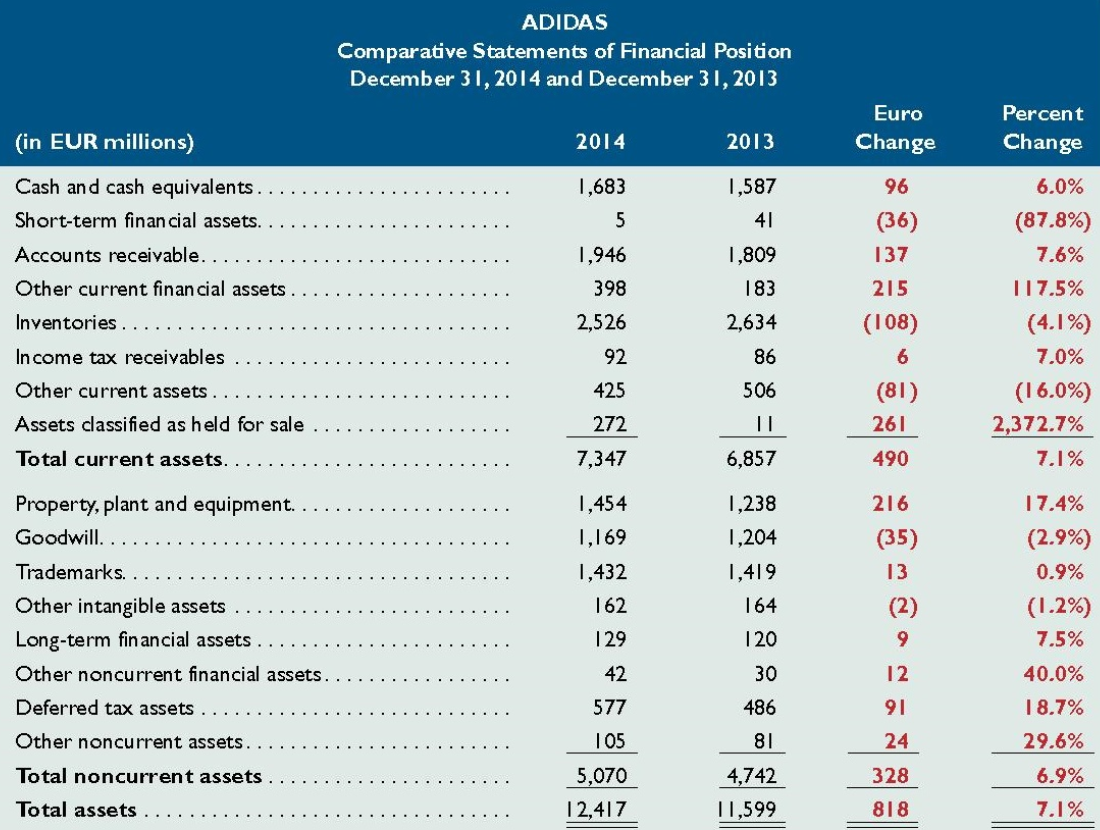
\includegraphics[width=\columnwidth]{images/c12/horizontal_analysis.png}
	\end{figure}

	To compare one year to another, the first task is to calculate the change 
	in dollar amount.  First, establish a base year (usually the prior year) 
	and then calculate the amount of change by comparing the analysis period to 
	the base period amount. The analysis period is usually the current year 
	while the base period is usually the prior year.
	\[
	\text{Dollar Change} = \text{Analysis Period Amount} - \text{Base Period 
	Amount}
	\]
	To calculate the amount of change as a percentage, divide the amount of the 
	dollar change by the base period amount, and then multiply by 100 to 
	convert to a percentage. 
	\[
	\text{Percent Change} = \frac{\text{Dollar Change}}{\text{Base Period 
	Amount}} \times 100
	\]
	This process is completed for each line item on the statement of financial 
	position.
	
	\subsubsection{Trend Analysis}
	
	Trend analysis, also called \textbf{trend percent analysis} or 
	\textbf{index number trend analysis}, is a form of horizontal analysis that 
	can reveal patterns in data across successive periods. It involves 
	computing trend percents for a 
	series of financial numbers and is a variation on the use of percent 
	changes. The difference is that trend analysis does not subtract the base 
	period amount in the numerator. To compute trend percents, we do the 
	following:
	\begin{enumerate}[noitemsep]
		\item Select a base period and assign the base period a weight of 100\%.
		\item Express financial numbers as a percent of the base period number.
	\end{enumerate}
	All values will be expressed as a percentage increase or decrease from the 
	base period. The base period is usually the oldest period shown.
	\[
	\text{Trend Percent} = \frac{\text{Analysis Period Amount}}{\text{Base 
	Period Amount}} \times 100
	\]
	\begin{figure}[ht]
		\centering
		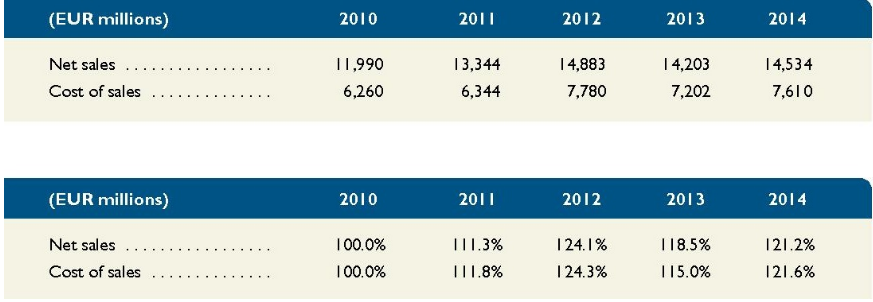
\includegraphics[width=\columnwidth]{images/c12/trend_analysis.png}
	\end{figure}
	
	Some managers prefer to review trend information in chart form. Using Excel 
	is an easy way to develop charts from our data.
	
	\subsubsection{Vertical Analysis}
	
	Vertical analysis is a tool to evaluate individual financial statement 
	items or a group of items in terms of a specific base amount. We usually 
	define a key aggregate figure as the base, which for an income statement is 
	usually revenue and for a statement of financial position is usually total 
	assets.
	
	The term vertical analysis arises from the up-down (or down-up) movement of 
	our eyes as we review common-size financial statements. Vertical analysis 
	is also called \textbf{common-size analysis}.
	\[
	\text{Common-size Percent} = \frac{\text{Analysis Amount}}{\text{Base 
	Amount}} \times 100
	\]
	\begin{figure}[ht!]
		\centering
		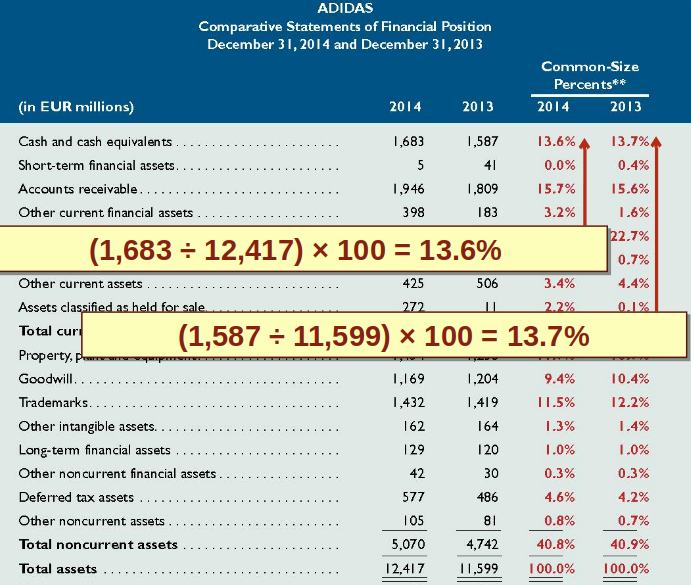
\includegraphics[width=\columnwidth]{images/c12/vertical_analysis1.png}
		\caption{Each line item is expressed as a percentage of total 
		assets.}  	
	\end{figure}
	
	For common-sized Income Statements, each item can be represented as a 
	percentage of net sales.
	
	\subsection{Ratio Analysis}
	
	Ratios are among the more widely used tools of financial analysis because 
	they provide clues to and symptoms of underlying conditions. A ratio can 
	help us uncover conditions and trends difficult to detect by inspecting 
	individual components making up the ratio. Ratios, like other analysis 
	tools, are usually future oriented; that is, they are often adjusted for 
	their probable future trend and magnitude, and their usefulness depends on 
	skillful interpretation.
	
	A ratio expresses a mathematical relation between two quantities. It can be 
	expressed as a percent, rate, or proportion. he ratios are organized into 
	the four building blocks of financial statement analysis:
	\begin{itemize}[noitemsep]
		\item \textbf{liquidity and efficiency}
		\item \textbf{solvency}
		\item \textbf{profitability}
		\item \textbf{market prospects}
	\end{itemize}
	
	\subsubsection{Liquidity and Efficiency}
	
	\textbf{Liquidity} refers to the availability of resources to meet 
	short-term cash 
	requirements. It is affected by the timing of cash inflows and outflows 
	along with prospects for future performance. Analysis of liquidity is aimed 
	at a company’s funding requirements. 
	
	\textbf{Efficiency} refers to how productive a 
	company is in using its assets. Efficiency is usually measured relative to 
	how much revenue is generated from a certain level of assets.
	
	\paragraph{Working capital.} Work Capital is defined as current assets 
	minus current liabilities.  It 
	is a critical measure for all types of businesses.  Positive working 
	capital means the company will have enough assets converted into cash 
	within the next year to pay its current obligations. 
	\[
	\text{Work Capital} = \text{Current Assets} - \text{Current Liabilities}
	\]
	
	\paragraph{Current Ratio.} It is merely current assets divided by current 
	liabilities.
	\[
	\text{Current Ratio} = \frac{\text{Current Assets}}{\text{Current 
	Liabilities}}
	\]
	As a short-term creditor, you would be vitally interested in a company’s 
	current ratio. If the ratio continues to lower over time, you may be less 
	likely to be paid in full. A higher current ratio suggests a strong 
	liquidity position and an ability to meet current obligations.
	
	\paragraph{Acid Test Ratio.} The acid-test ratio is a more stringent 
	measure 
	than the current ratio.  We calculate the ratio by dividing quick assets by 
	current liabilities. Quick assets include cash, short-term investments, and 
	current accounts and notes receivable.
	\[
	\text{Quick Assets}= \text{Cash} + \text{Short-term Financial Assets} - 
	\text{Current Receivables}
	\]
	\[
	\text{Acid-test Ratio} = \frac{\text{Quick Assets}}{\text{Current 
	Liabilities}}
	\]
	The acid test ratio is generally lower than the current ratio because we 
	have reduced the numerator. We have removed inventory accounts from the 
	numerator that generally require a period of time to convert into cash.
	
	\paragraph{Accounts Receivable Turnover.} This ratio measure how many times 
	a company converts its receivables into cash each year. We calculate 
	accounts receivable turnover by dividing our net credit sales, or sales on 
	account, by average accounts receivable. 
	\[
	\text{Account Receivable Turnover} = \frac{\text{Net Sales}}{\text{Average 
	Accounts Receivable}}
	\]
	This is an example of a ratio that contains an income statement measure in 
	the numerator and a statement of financial position measure in the 
	denominator. Remember, in this type of ratio, we always use an average 
	amount in the denominator. Our average accounts receivable, net is equal to 
	the beginning accounts receivable plus the ending accounts receivable and 
	the total divided by 2. For any company, the higher the turnover, the 
	faster the cash collection on accounts receivable.
	
	\paragraph{Inventory Turnover.} The inventory turnover ratio measures the 
	number of times inventory is sold and replaced during the year. Inventory 
	turnover is calculated by dividing cost of goods sold for the period by the 
	average inventory. 
	\[
	\text{Average Inventory} = \frac{\text{Cost of Goods Sold}}{\text{Average 
	Inventory}}
	\]
	Higher inventory turnover helps protect a company from obsolete inventory 
	items.
	
	\paragraph{Accounts Payable Turnover.} A short-term liquidity measure used 
	to quantify the rate at which a company pays off its supplies. 
	\[
	\text{Accounts Payable Turnover} = \frac{\text{Cost of Goods 
	Sold}}{\text{Average Accounts Payable}}
	\]
	
	Inventories 
	are often financed by accounts payable. Such payables usually represent 
	interest-free financing and are therefore less expensive than using 
	borrowed money to finance inventory purchases or production.
	
	\paragraph{Days' Sales Uncollected.} Days’ sales uncollected is calculated 
	by dividing ending accounts receivable, net by net sales, and multiplying 
	this amount by 365 days. 
	\[
	\text{Days' Sales Uncollected} = \frac{\text{Accounts 
	Receivable, Net}}{\text{Net Sales}} \times 365
	\]
	If a company offers a two-ten, net thirty cash discount, many customers 
	would pay off the receivable balance close to the ten-day discount period 
	and reduce the days’ sales uncollected ratio. 
	
	\paragraph{Days' Sales In Inventory.}  Days’ sales in inventory by dividing 
	ending inventory by cost of goods sold, and multiplying this amount by 365 
	days. 
	\[
	\text{Days' Sales In Inventory} = \frac{\text{Ending Inventory}}{\text{Cost 
	of Goods Sold}} \times 365
	\]
	This ratio is a useful measure in evaluating inventory liquidity. If a 
	product is demanded by customers, this formula estimates how long it takes 
	to sell the inventory. The greater the demand for the product, the quicker 
	it will be sold. By combining information about the days’ sales in 
	inventory and the accounts receivable turnover, we get additional insights 
	about the sale of a product and the collection of the related receivable 
	into cash.
	\paragraph{Days' Purchases in Accounts Payable.} This ratio is a useful 
	measure in evaluating how long the business takes to pay its credit 
	suppliers.
	\[
	\text{Days' Purchase In Accounts Payable} = \frac{\text{Accounts 
	Payable}}{\text{Cost of Goods Sold}} \times 365
	\]
	
	\paragraph{Cash Conversion Cycle.} The cash conversion cycle of a company 
	is defined by the sum of the days’ sales uncollected and the days’ sales in 
	inventory subtracting the days’ purchases in accounts payable.
	
	It represents the number of days a firm’s cash remains tied up within the 
	operations of the business. It is also a powerful tool for assessing how 
	well a company is man- aging its working capital. The lower the cash 
	conversion cycle, the more healthy a company generally is.
	
	\paragraph{Total Asset Turnover.} Total asset turnover is equal to net 
	sales divided by average total assets.
	\[
	\text{Total Asset Turnover} = \frac{\text{Net Sales}}{\text{Average Total 
	Assets}}
	\]
	Asset turnover is a measure of how efficiently management is using the 
	available assets to generate sales.
	
	\subsubsection{Solvency}
	
	Solvency refers to a company’s long-run financial viability and its ability 
	to cover long-term obligations. One of the most important components of 
	solvency analysis is the composition of a company’s capital structure. 
	\textbf{Capital structure} refers to a company’s financing sources.
	
	\paragraph{Debt Ratio.} Debt ratio measures what portion of a company’s 
	assets are contributed by creditors. A larger debt ratio implies less 
	opportunity to expand through use of debt financing. The debt ratio 
	expresses total liabilities as a percent of total assets. 
	\[
	\text{Debt Ratio} = \frac{\text{Total Liabilities}}{\text{Total Assets}} 
	\times 100\%
	\]
	
	\paragraph{Equity Ratio.} The equity ratio provides complementary 
	information by expressing total equity as a percent of total assets.
	\[
	\text{Equity Ratio} = \frac{\text{Total Equity}}{\text{Total Assets}} 
	\times 100\%
	\]
	
	\paragraph{Debt-to-Equity Ratio.} This ratio measures what portion of the 
	company's assets are contributed by creditors. 
	\[
	\text{Debt-to-Equity Ratio} = \frac{\text{Total Liabilities}}{\text{Total 
	Equity}}
	\]
	
	A calculation above one indicates the 
	company has more liabilities than equity. The lower the calculation, the 
	more solvency the company has. A larger debt-to-equity ratio implies less 
	opportunity to expand through use of debt financing.
	
	\paragraph{Times Interest Earned.} Long-term creditors are particularly 
	interested in the ability of a company to meet periodic interest payments. 
	Times interest earned is a ratio that would be important to long-term 
	creditors.  The ratio is calculated by dividing earnings before interest 
	and taxes by interest expense for the period. 
	\[
	\text{Times Interest Earned} = \frac{\text{Profit before interest expense 
	and income tax}}{\text{Interest Expense}}
	\]
	The larger the ratio, the less risky the company is from the perspective of 
	a long-term creditor.
	
	\subsubsection{Profitability}
	
	Profitability refers to a company’s ability to generate an adequate return 
	on invested capital. Return is judged by assessing earnings relative to the 
	level and sources of financing. Key profitability measures are profit 
	margin, return on total assets, earnings per share and return on ordinary 
	shareholder’s equity.  
	
	\paragraph{Profit Margin.} Profit margin tells us how effective the company 
	is at producing bottom line net profit.  The ratio is determined by 
	dividing net profit by net sales.
	\[
	\text{Profit Margin} = \frac{\text{Net Profit}}{\text{Net Sales}}
	\] 
	
	\paragraph{Return on Total Assets.} We can determine the return a company 
	earns on its total assets.  To 
	calculate this ratio, we divide net profit by the average total assets for 
	the period. 
	\[
	\text{Return on Assets} = \frac{\text{Net Profit}}{\text{Average Total 
	Assets}}
	\]
	Return on total assets measures how well assets have been 
	employed by the company’s management. 
	
	\paragraph{Return on Ordinary Shareholders' Equity.} The numerator is net 
	profit available to ordinary shareholders, which is net profit less 
	preference dividends, divided by average ordinary shareholders’ equity. 
	
	\begin{equation}
	\begin{aligned}
	\text{Return on Ordinary Shareholders' Equity} \\=\frac{\text{Net Profit - 
	Preference Dividends}}{\text{Average Ordinary Shareholders' Equity}}
	\end{aligned}
	\end{equation}
	This measure indicates how well the company employed the shareholders’ 
	equity to earn net profit.
	
	
	\paragraph{Earnings Per Ordinary Share (EPS).} This shows the amount of net 
	income 
	earned for each outstanding ordinary share. It is the most widely used 
	ratio and it is calculated by dividing net income by the weighted average 
	number of ordinary shares outstanding during the year.

	\begin{equation}
	\begin{aligned}
	&\text{Earnings per Ordinary Share} \\&=\frac{\text{Net Income - 
			Preference Dividends}}{\text{Weighted Average number of ordinary 
			shares outstanding}}
	\end{aligned}
	\end{equation}
	
	\subsubsection{Market Measures}
	
	Market measures are useful for analyzing corporations with publicly traded 
	shares. These market measures use share price, which reflects the market’s 
	(public’s) expectations for the company. This includes expectations of both 
	company return and risk—as the market perceives it.  Key measures of market 
	prospects include the price-earnings ratio and dividend yield.
	
	\paragraph{Price-Earnings Ratio.} This measures is often used by investors 
	as a general guideline in gauging share values. Generally, the higher the 
	price-earnings ratio, the more opportunity a company has for growth. Once 
	we know the earnings per share, we can calculate the price-earnings ratio, 
	or PE ratio.  We will divide the closing market price per share of a 
	company’s ordinary shares by earnings per share
	\[
	\text{Price-to-Earnings Ratio} = \frac{\text{Market Price per ordinary 
	Share}}{\text{Earnings per share}}
	\]
	The ratio is used as an indicator of the future growth and risk of a 
	company’s earnings as perceived by the share’s buyers and sellers.
	
	
	\paragraph{Dividend Yield.} If you are an investor who requires current 
	income; you will want to look for companies with high dividend payout 
	ratios.  If you believe that a company can invest its funds and earn a 
	higher return than you would be able to earn, you might look for a company 
	with high growth and a low payout ratio. To determine the dividend yield 
	ratio, we divide the annual dividend per share by the closing market price 
	per share of the company’s ordinary shares. 
	\[
	\text{Dividend Yield} = \frac{\text{Annual Cash Dividend Per 
	Share}}{\text{Market Price per Share}}
	\]
	
	\subsection{Factors Contributing to Going-Concern PRoblems}
	
	\begin{figure}[ht]
		\centering
		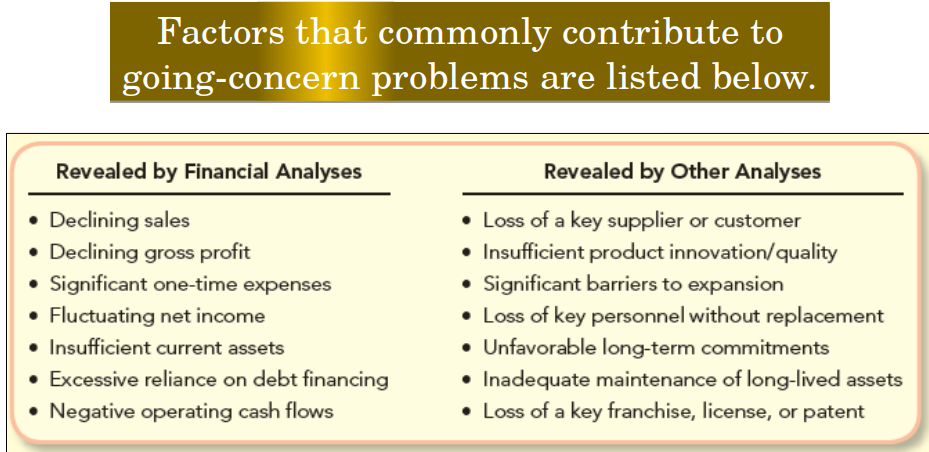
\includegraphics[width=\columnwidth]{images/c12/going_concern.png}
	\end{figure}

	If ever a company encounters a going-concern problem, it may need to adjust 
	the amount and classification of items in its financial statements, which 
	would be explained in the financial statement notes and to which the 
	auditor’s report would draw attention. Financial and other types of 
	analyses often call to our attention a potential going-concern issue.

\end{document}